\documentclass[utf8,13pt]{beamer}
%\usepackage{cmap}
\usepackage{amsmath,amssymb}
\usepackage{helvet}

\usepackage{nicefrac}
\usepackage{rotating}

\usetheme[numbering=fraction,block=fill]{metropolis}
\setbeamerfont{frame footer}{size=\tiny}
\setbeamerfont{page number in head/foot}{size=\tiny}
\setbeamerfont{title}{size=\large}
\setbeamertemplate{frame footer}{\insertshortauthor~-- \insertshorttitle}
\setbeamercolor{footline}{fg=gray}

%\usefonttheme{professionalfonts}
\setbeamertemplate{bibliography item}{}
\setbeamertemplate{navigation symbols}{}
\setbeamertemplate{blocks}[rounded]
% Use I,II,III for numbering in frametitle with framebreaks
\setbeamertemplate{frametitle continuation}{[\insertcontinuationcount]}

%% \usepackage{pgfpages}
%% \pgfpagesuselayout{6 on 1}[a4paper,border shrink=5mm]

%\usepackage{ulem}
%\renewcommand{\ULthickness}{1.5pt}

%% show current section/subsection in footer (as small normal text)
%% \usetheme{boxes}
%% \addfootbox{normal text}{\tiny\qquad\insertsectionhead}

%\usefonttheme{default}
%\usefonttheme{structurebold}
%\setbeamerfont{block title}{size={}}

%% make black-and-white
%\setbeamercolor{structure}{fg=black}
%\setbeamercolor{block body}{bg=white}
%\setbeamercolor{title}{fg=structure.bg,bg=structure.fg}
%\setbeamercolor{alerted text}{fg=normal text.fg}
%\setbeamerfont{alerted text}{shape=\itshape}

% make margins a bit smaller
\setbeamersize{text margin left=.75cm}
\setbeamersize{text margin right=.75cm}

%% less indentation in sublists
% \setlength{\leftmargini}{1em}
% \setlength{\leftmarginii}{0.75em}
% \setlength{\leftmarginiii}{0.75em}
% \setlength{\labelsep}{.5em}
% \setlength{\labelwidth}{1em}
%
\setbeamerfont{itemize/enumerate subbody}{size=\normalsize}
\setbeamerfont{itemize/enumerate subsubbody}{size=\normalsize}
\setbeamerfont{itemize/enumerate subitem projected}{size=\normalsize}
\setbeamerfont{itemize/enumerate subsubitem projected}{size=\normalsize}
%
% \setbeamertemplate{itemize item}{\textbf{\texttt{*}}}
% \setbeamertemplate{itemize subitem}{\texttt{>}}
% \setbeamertemplate{itemize subsubitem}{\texttt{-}}
%
% \setbeamertemplate{enumerate item}{\textit{\insertenumlabel}.~}

%% no navigation symbols
%\setbeamertemplate{navigation symbols}{}
%% \setbeamercovered{dynamic}
%\setbeamercovered{transparent=70}

%\definecolor{anugray}{rgb}{0.259,0.259,0.259}
%\setbeamercolor{inverted}{fg=white,bg=anugray}

\usepackage{tikz}
\usetikzlibrary{snakes}
\usetikzlibrary{arrows}
\usetikzlibrary{patterns}

\newcommand{\set}[1]{\{#1\}}
\newcommand{\suchthat}{\,|\,}
\newcommand{\ptype}[1]{\texttt{#1}}

\newcommand{\length}{\operatorname{len}}
\newcommand{\cost}{\operatorname{cost}}

\setlength{\tabcolsep}{2mm}
\setlength{\arraycolsep}{0mm}
%\setlength{\eqnindent}{0mm}

\makeatletter
\setbeamertemplate{frametitle}{%
  \nointerlineskip%
  \begin{beamercolorbox}[%
      wd=\paperwidth,%
      sep=0pt,%
      leftskip=\metropolis@frametitle@padding,%
      rightskip=\metropolis@frametitle@padding,%
    ]{frametitle}%
  \metropolis@frametitlestrut@start%
  \insertframetitle%
  \nolinebreak%
  \metropolis@frametitlestrut@end%
  \hfill
  %\raisebox{-0.6ex}{\includegraphics[height=3ex,keepaspectratio]{anu_logo}}
  \end{beamercolorbox}%
}
\makeatother



\pdfinfo{
/Title (Narrative Planning: Planning with a Theory of Mind)
/Author (...)
}

\begin{document}

\title{Planning with a Theory of Mind}
\institute{}
\author{ICAPS Tutorial: Narrative Planning}
\date{ICAPS 2024}

\frame[label=intro,plain,noframenumbering]{\titlepage}

%%%%%%%%%%%%%%%%%%%%%%%%%%%%%%%%%%%%%%%%%%%%%%%%%%%%%%%%%%%%%%%%%%%%%%

\begin{frame}{Planning with a Theory of Mind}
  \begin{columns}
    \begin{column}{.62\linewidth}
      \begin{itemize}
      \item \textit{Theory of Mind}: the capacity to understand others
        have a mind of their own, and reason about what goes on in it.
      \item To be believable, characters must behave consistently
        with what an audience believes is in their minds.
        %% and therefore the author must reason about what characters
        %% are thinking
      \item Characters may need to reason about what other characters
        want, believe, and intend.
        %% when that is what the audience expects them to do!
      \end{itemize}
    \end{column}
    \begin{column}{.315\linewidth}
      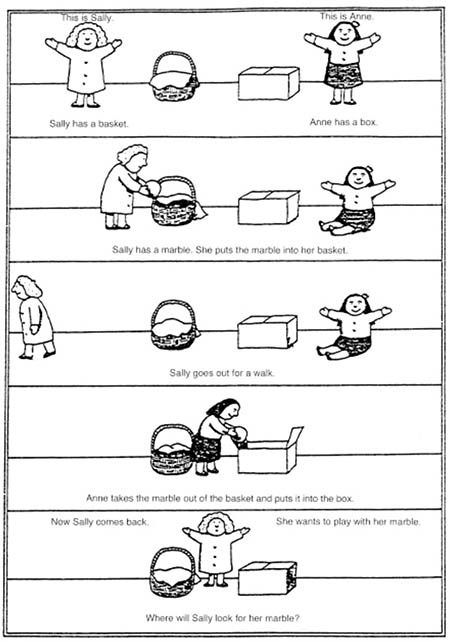
\includegraphics[width=\linewidth]{sally_anne_test.jpg}\\
      \begin{minipage}{\linewidth}
        \tiny
        (Baron-Cohen, Leslie and Frith 1985)\\
        \url{https://en.wikipedia.org/wiki/Sally\%E2\%80\%93Anne_test}
      \end{minipage}
    \end{column}
  \end{columns}
\end{frame}

\begin{frame}
  \begin{itemize}
  \item Planning from the author's perspective:
    \begin{itemize}
    \item Must reason about what characters want, believe and plan,
      to preserve the illusion that characters are planning and acting
      of their own will.
    \item May reason about what characters believe or assume about
      what other characters want, believe and plan (because that is
      what we do)
    \item May reason about what the audience believes,
      to create dramatic effect.
    \end{itemize}
  \item Planning from a character's perspective:
    \begin{itemize}
    \item Must work from the beliefs and goals the character has
      (or is intended or perceived to have).
    \item May reason about what other characters want, believe
      and plan, to predict or manipulate their actions.
    \end{itemize}
  \end{itemize}
\end{frame}

\begin{frame}{Intentionality}
  %\framesubtitle{(Riedl \& Young 2010)}
  \begin{itemize}
  \item Riedl \& Young (2010) distinguish \emph{intentional} actions,
    performed by one or more characters (its \emph{actors}), from
    non-volitional events.
  \item A plan is \emph{intentional} iff every intentional action
    contributes, directly or indirectly, to achieve an intention (goal)
    of the character(s) who perform it.
  \item Characters can acquire intentions as an effect of events or other
    characters' actions, depending on their character traits.
    %% \begin{itemize}
    %% \item For example, when the king hears about a treasure, he acquires
    %%   the goal of owning it because he is greedy, and
    %% \item when the king orders his knight to get him the treasure, the
    %%   knight acquires the same goal because he is obedient.
    %% \end{itemize}
  \end{itemize}
\end{frame}

\begin{frame}
  \begin{itemize}
  \item Formalised by Riedl \& Young in the context of POCL plans.
  \item A \emph{frame of commitment} is a subset $S'$ of plan steps
    such that:
    \begin{itemize}
    \item character $A$ is an actor of every step in $S'$;
    \item there is a \emph{final step} $s_{fin} \in S'$ that adds $g$;
    \item there is a \emph{motivating step} $s_m$ that adds
      \ptype{(intends $A$ $g$)} and that preceds all steps in $S'$; and
    \item for each step in $S'$ other than $s_{fin}$ there is a path of
      causal and/or motivational links to $s_{fin}$.
    \end{itemize}
  \item A plan is \emph{intentional} iff every intentional action with
    actor $A$ belongs to a frame of commitment of $A$.
  %% \item This can implemented in several ways:
  %%   \begin{itemize}
  %%   \item modified POCL algorithm (Rield \& Young 2010);
  %%   \item modification of heuristic state-space search (Ware 2012);
  %%   \item reformulation into classical planning (Haslum 2012).
  %%   \end{itemize}
  \end{itemize}
\end{frame}

\begin{frame}{Conflict}
  %\framesubtitle{(Ware \& Young 2011)}
  \begin{itemize}
  \item Riedl \& Young's definition does not allow plans in which
    characters \emph{fail}, either because
    \begin{itemize}
    \item they planned from mistaken beliefs; or
    \item another character's actions thwarted their plan.
    \end{itemize}
  \item Ware \& Young (2011) amend the definition of intentional
    plans to allow for plans with inter-character \emph{conflict},
    by allowing characters' plan, while complete, to be only partially
    executed.
  \item Formally, they distinguish between \emph{executed} and
    \emph{non-executed} steps in the plan:
    \begin{itemize}
    \item both executed and non-executed steps may be used to complete
      a frame of commitment; but
    \item only executed steps are subject to normal plan validity.
    \end{itemize}
  \end{itemize}
\end{frame}

\begin{frame}{Belief}
  \begin{itemize}
  \item Representing character \emph{beliefs} about the world state
    means representing a potentially different state for each character.
  \item Character's beliefs can change as a consequence of
    \begin{itemize}
    \item their actions (failure uncovers false belief);
    \item other character's actions (telling or revealing); and
    \item non-volitional events (observation).
    \end{itemize}
  \item Formalised (\textit{e.g.}, Teutenberg \& Porteous 2015; Christensen
    et al.\ 2020):
    \begin{itemize}
    \item Character's plans (frames of intention) must be complete with
      respect to the facts that the character believes.
    \item Requires modelling the effects of a character attempting an
      action whose preconditions are in fact not true.
    \end{itemize}
  \end{itemize}
\end{frame}

\begin{frame}
  \begin{itemize}
  \item Although properties like intentionality, conflict, belief are
    often formalised in the context of (extended) POCL plans, planners
    achieving them can be \emph{implemented} in many ways, \textit{e.g.}:
    \begin{itemize}
    \item By modification/extension of classical POCL algorithms
      (Riedl \& Young 2010; Ware \& Young 2011).
    \item By modification/extension of (heuristic) state-space
      search planners (Ware 2012; Ware \& Young 2014;
      Sanghrajka et al.\ 2022).
    \item Through multi-agent planning (Brenner 2010;
      Teutenberg \& Porteous 2013, 2015; Porteous \& Lindsay 2019).
    \item By reformulation/compilation (Haslum 2012; Christensen
      et al.\ 2020).
    \end{itemize}
  \end{itemize}
\end{frame}

\begin{frame}{Planner as an Audience Model}
  \begin{itemize}
  \item A planner, using the facts of the story narrated so far, can
    be used as a model of the audience's expectations:
    \begin{itemize}
    \item If there are few or unlikely plans in which the story's
      protagonist is successful from the current state, then the
      state is \emph{suspenseful}
      (O'Neill \& Riedl 2014; Cheong \& Young, 2015).
    \item If the story diverges from the plan generated by the
      audience model, then the story is \emph{surprising}
      (Bae \& Young, 2014).
    \end{itemize}
  \item Can also incorporate reasoning about the audience's likely
    inferences from narrated facts (\textit{e.g.}, Arinbjarnar 2008;
    Chieppe et al.\ 2022).
  \end{itemize}
\end{frame}

%% \begin{frame}{Conclusion}
%%   \begin{itemize}
%%   \item ...
%%     \begin{itemize}
%%     \item ...
%%     \item ...
%%     \end{itemize}
%%   \item ...
%%   \end{itemize}
%% \end{frame}

\begin{frame}{References}
  \footnotesize
  \begin{itemize}
  \item Maria Arinbjarnar (2008). Dynamic Plot Generating Engine.
    Workshop on Integrating Technologies for Interactive Stories
    \url{http://www-users.cs.york.ac.uk/~maria/greinar/dpge.pdf}.
  \item Byung-Chull Bae, R. Michael Young  (2014).
    A Computational Model of Narrative Generation for Surprise Arousal.
    IEEE Transactions on Computational Intelligence and AI in Games,
    vol.\ 6(2).
  %%\item Baron-Cohen, Leslie \& Frith (1985)
  \item Brenner (2010).
    Creating Dynamic Story Plots with Continual Multiagent Planning.
    AAAI.
  \item Yun-Gyung Cheong, R. Michael Young (2015).
    Suspenser: A Story Generation System for Suspense.
    IEEE Transactions On Computational Intelligence and AI in Games,
    vol.\ 7(1).
  \item Patrick Chieppe, Penny Sweetser, Eryn Newman (2022).
    Bayesian Modelling of the Well-Made Surprise. ICCC.
  \end{itemize}
\end{frame}

\begin{frame}
  \footnotesize
  \begin{itemize}
  \item Matthew Christensen, Jennifer M. Nelson, Rogelio E. Cardona-Rivera
    (2020).
    Using Domain Compilation to Add Belief to Narrative Planners. AIIDE.
  \item Patrik Haslum (2012).
    Narrative Planning: Compilations to Classical Planning.
    JAIR vol.\ 44.
  \item Brian O'Neill and Mark Riedl (2014).
    Dramatis: A Computational Model of Suspense. AAAI.
  \item Julie Porteous, Alan Lindsay (2019).
    Protagonist vs Antagonist PROVANT: Narrative Generation as Counter
    Planning. AAMAS.
  \item Mark O. Reidl and R. Michael Young (2010).
    Narrative Planning: Balancing Plot and Character.
    JAIR.
  \item Rushit Sanghrajka, R. Michael Young, Brandon Thorne (2022).
    HeadSpace: Incorporating Action Failure and Character Beliefs into
    Narrative Planning. AIIDE.
  \item Jonathan Teutenberg and Julie Porteous (2013).
    Efficient Intent-Based Narrative Generation Using Multiple Planning
    Agents. AAMAS.
  \end{itemize}
\end{frame}

\begin{frame}
  \footnotesize
  \begin{itemize}
  \item Jonathan Teutenberg and Julie Porteous (2015).
    Incorporating Global and Local Knowledge in Intentional Narrative
    Planning.
  \item Stephen G. Ware, Robert Michael Young (2011).
    CPOCL: A Narrative Planner Supporting Conflict. AIIDE.
  \item Stephen G. Ware (2012).
    The Intentional Fast-Forward Narrative Planner.
    Workshop on Intelligent Narrative Technologies @ AIIDE.
  \item Stephen G. Ware, Robert Michael Young (2014).
    Glaive: A State-Space Narrative Planner Supporting Intentionality
    and Conflict. AIIDE.
  \end{itemize}
\end{frame}

\end{document}
